\chapter{Results}

\section{Resnet}

% \subsection{Linear evaluation on features}

The following Figure~\ref{fig:spider_resnet50} shows the result with Resnet50, while Table~\ref{tab:f1_scores_resnet_derma} and Table~\ref{tab:f1_scores_resnet_plant} contain the respective values.
\begin{figure}[H]
    \begin{center}
    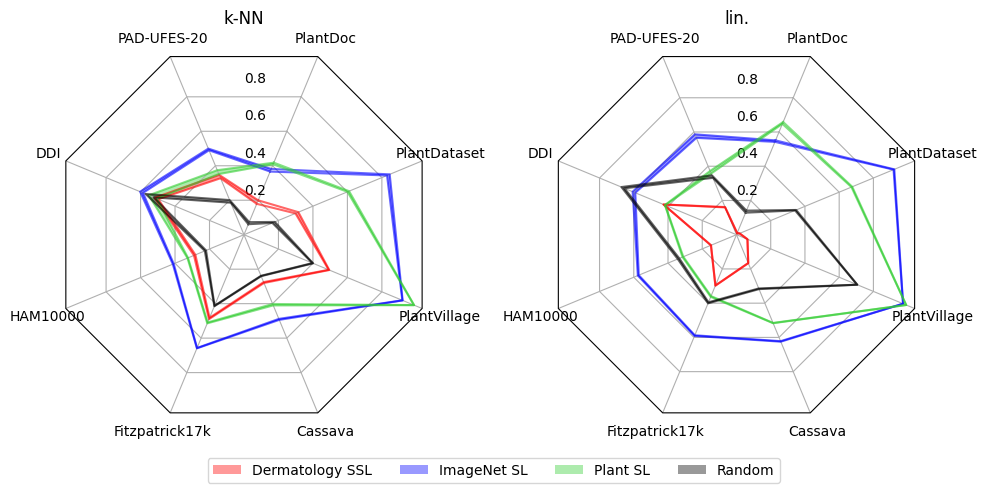
\includegraphics[width=15cm]{spider_resnet50.png}
    \caption{Linear evaluation of Resnet50}\label{fig:spider_resnet50}
    \end{center}
\end{figure}

The first thing to notice is the awful performance of the model trained on dermatology with SimCLR. The scores are never significantly better than the other pre-trained models. The model which was trained on ImageNet with \gls{ssl} was not put into the graphic, but the tables show that these scores are bad as well. 
This indicates a problem with the type of training rather than with the data per se.

In the linear evaluation the plant based model is actually a bit better than the ImageNet based model, but with \gls{knn} the difference becomes negligible.



\section{Vision Transformers}

The results of the \gls{vit} can bee seen in Figure~\ref{fig:spider_vit}, Table~\ref{tab:f1_scores_vit_derma} and Table~\ref{tab:f1_scores_vit_plant}. 
The scores look similar. The scores of the plant based model are better in some tasks than the model trained with \gls{sl} on ImageNet, but not better than the \gls{ssl} variant. All DINO based models are relatively close to each other. This is probably due to their way of training rather than the data.

\begin{figure}[H]
    \begin{center}
    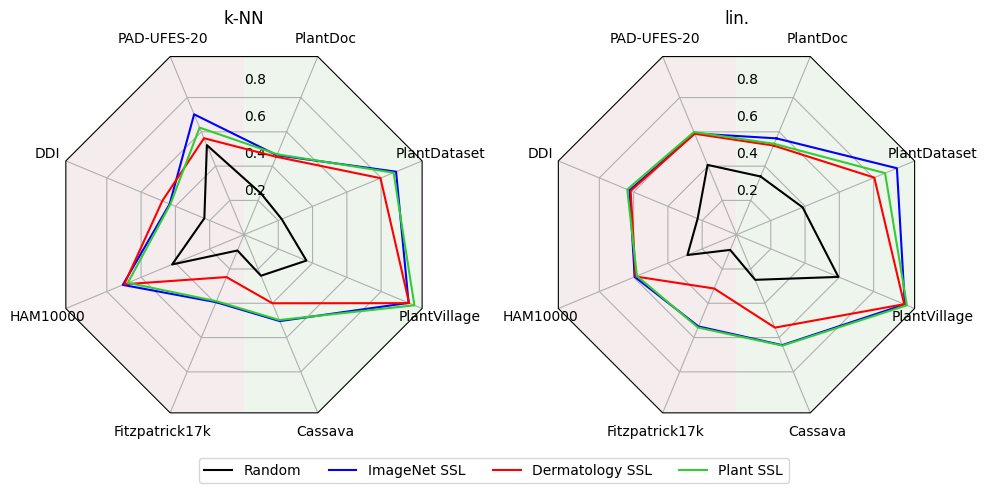
\includegraphics[width=15cm]{spider_vit.png}
    \caption{Linear evaluation of \gls{vit}}\label{fig:spider_vit}
    \end{center}
\end{figure}




% \subsection{Subsampling}
% \section{Other}
% \subsection{DINO student/teacher}
% \subsection{Fine-tuning}
% \subsection{Fine-tuning}
